\section{Architecture}
\label{sec:architecture}

As shown in Figure \ref{fig:archi}, we have developed a Python framework, which is a high-level package of NAOqi APIs and ROS-based components. 
\begin{figure}[!h]
    \centering
    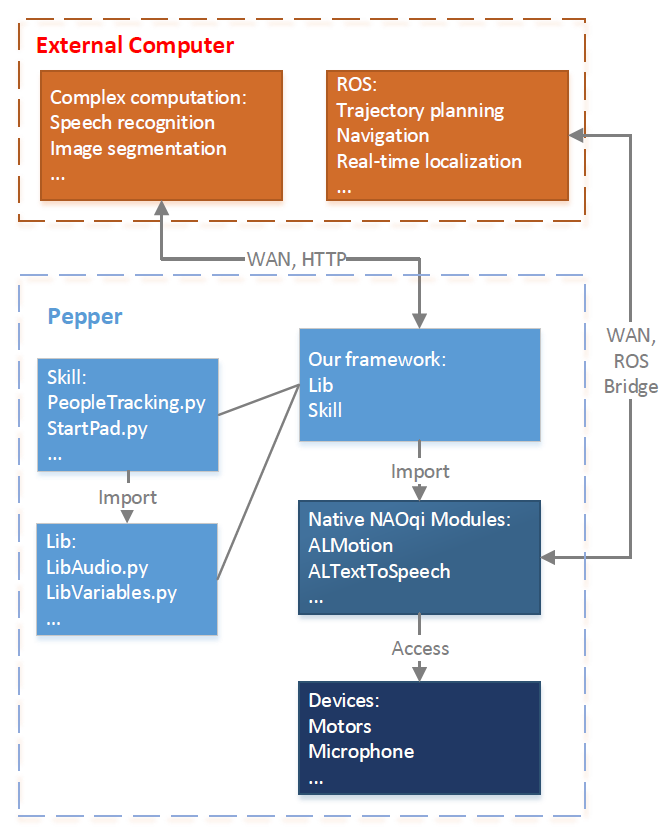
\includegraphics[width=4in]{figs/architecture.png}
    \caption{System architecture}
    \label{fig:archi}
\end{figure}

\subsection{NAOqi Operation System}
\label{subsec:naoqi}
In most aspects, NAOqi OS behaves like a Linux.
The most significant feature is its NAOqi modules.
Various modules can be accessed through network by the proxy called "ALBroker".
To upper level application, the proxy is transparent, which makes remote access has no difference with local access.
All underlying hardware can be used by these NAOqi modules easily.
Figure \ref{fig:naoqi} shows the NAOqi architecture.

\begin{figure}[!h]
    \centering
    \subfigure[File organization]{\label{fig11}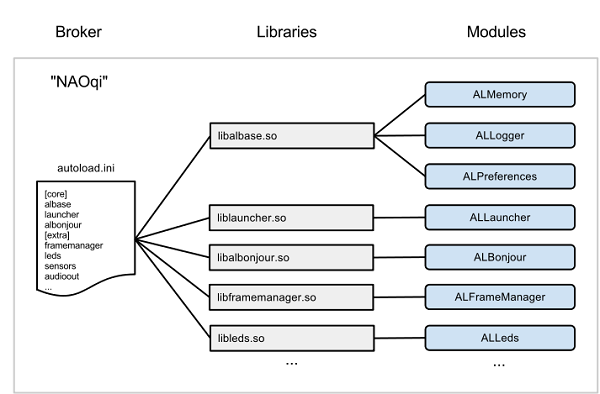
\includegraphics[width=2.5in]{figs/naoqi1.png}}
    \hspace{0.2in}
    \subfigure[Access process]{\label{fig12}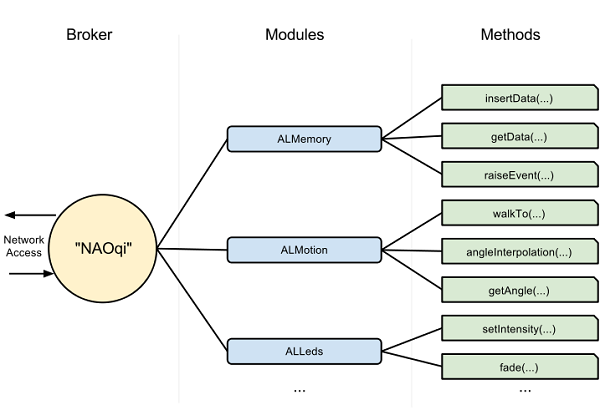
\includegraphics[width=2.5in]{figs/naoqi2.png}}
    \caption{NAOqi API}
    \label{fig:naoqi}
\end{figure}

\subsection{Homemade framework on Pepper}
\label{subsec:native}

On NAOqi OS, several processes are simultaneously running, including UI process, HTTP server/client process, motion control process, vision process, navigation process, etc.
All codes are organized into two main parts: libraries and skills. 
Libraries, we name them with “/Lib.*\.py/” pattern, are files that contain various class definitions for basic ablilities. 
Every “Lib” attaches to some specific functions. 
For example, “LibVariables” defines a class related to global variables stored on local disk or remote server. 
“Lib”s are just useful tools without any task-oriented purpose. 

To combine them together and implement specific applications, we write many app files, called “Skill”. 
A “Skill” imports several “Lib”s, to accomplish a complete task, such as tracking a person. 
Every “Skill” runs as an individual process, so communication problem follows. 
OS’s memory manager allocate different storage space for different processes, so there is no native global space for our different “Skill” and “Lib”. 
But most of time, there is a large need for them to share information. 
To overcome such dilemma, we developed a JSON-based global variable mechanism. As mentioned before, this function is implemented in “LibVariables”. 
It uses hard-disk to store a global variable with JSON format. 
Thanks to separation principle of interface and implementation, the global space can be not only Pepper local disk, but also remote server memory/disk. 

Overall, though many programs engaged, we just need to run a single shell script to start all applications we need. 
This native software system on Pepper is easy to learn, easy to use and easy to extend. 
Every team member can write his/her own lib files, such as "LibMoiton", "LibDetection", and add it to the framework by pushing their files to Pepper. 
The development process seems like building. It starts from a basic frame, and grows with bricks added by team members, and finally become a useful building.

\subsection{HTTP-based Information Exchange System}
\label{subsec:http}
Computational resources are limited in NAOqi OS. 
But in real applications quite a lot tasks need heavy computation, which require us to push them to a powerful remote computer.
So, we designed a HTTP-based information exchange system. There are two HTTP server process, one in Pepper, another in external computer. 

Main function of external computer server process is to listen to Pepper’s requests, start corresponding computing program and response the result to Pepper. 
A conspicuous example is speech recognition task. 
After recording a complex speech sentence from the operator, Pepper sends the audio file to the external computer through HTTP request. 
The computer receives this request, and converts this speech to text. 
Finally, speech text is sent back carried by HTTP response package. 

On the other hand, HTTP server process runs on Pepper mainly aims at web service. 
It contains a web site backend. 
When a browser login the URL, it gets a home page of various applications and can start them by simple clicks. 
Moreover, a device just need the ability of sending HTTP requests to control Pepper’s behavior. 

The advantage of HTTP information exchange is obvious, it is widely used and device/language independent. 
But network quality would limit the performance of HTTP communication. 
Future works contain compressing information to reduce transfer load.

\subsection{Robot Operation System (ROS)}
\label{subsec:ros}

Implementing SLAM and auto-navigation of robot needs well fusion of multi-sensor data and feedback control of motion actuators, so Robot Operating System (ROS) is a useful tool. 
We develop a basic module serving as a bridge between NAOqi and ROS, it publish Pepper’s sensor data in ROS format and enable ROS to call NAOqi’s APIs. 
ROS components get multi-sensor data, then do SLAM and path planning with real-time obstacle avoidance. 
As a result, motion commands will be sent to NAOqi.